% !TEX root =  master.tex 
\chapter{Mockup des UIs mit html -- Daniel Pies}

\section{Übersicht}

Unser zweites Mockup des Spiels haben wir mit html erstellt, um es mithilfe eines Webservers aufrufen zu können, da auch unser Spiel mittels eines Webservers auf verschiedenen Geräten gestartet werden kann. Das Mockup sollte alle Informationen erhalten, die der Spieler auch im fertigen Spiel als Entscheidungshilfe haben soll. Dazu bietet es sich an ein Grid-Layout zu verwenden, das mehrere Elemente auch nebeneinander anzeigen kann. Die html-Seite besteht hauptsächlich auch drei Spalten, wobei der Bereich der Spielereingaben noch einmal in drei Spalten unterteilt ist.


\begin{minipage}{\linewidth}
	\centering
	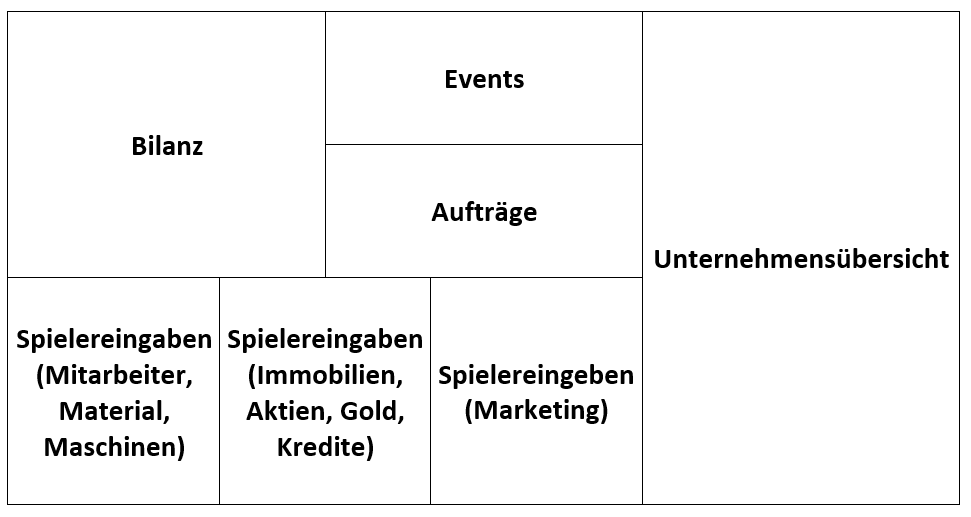
\includegraphics[scale=0.6]{img/Uebersicht.png}
	\captionof{figure}{\label{abb:aufbauhtml}Aufbau des html-Mockups}
	\vspace{1em}
\end{minipage}

\newpage

\section{Die wichtige Elemente}

Die wichtigen Elemente im UI sind:

\begin{description}
	\item[Die Übersicht]\hfill \\
	Hier sieht der Spieler die kompletten Informationen zu seinem Unternehmen. Alle Werte wie Kontostand, Immobilien, Bauarbeiter, Verwaltungsangestellte, Baumaschinen, Baumaterialen, Aktien, Gold, Kredite, Marketingscore und alle aktiven Baustellen sind detailliert aufgelistet.
	\item[Die Bilanz]\hfill \\
	Hier findet der Spieler die Bilanz seines Unternehmens analog zur Finanzbuchhaltung. Der Spieler hat einen finanziellen Überblick und sieht, ob er beispielsweise Investieren kann oder knapp bei Kasse ist.
	\item[Die Events]\hfill \\
	Hier stehen informative Texte zur letzter Runde, die den Spieler bei der nächsten Runde unterstützen können. Solche Texte sind zum Beispiel \glqq Das letzte Jahr war sehr erfolgreich. Die Wirtschaft erlebt einen deutlichen Aufschwung. Die Auftragslage ist weiterhin sehr gut.\grqq \ oder \glqq Im Stadtteil Eastside gab es einen Wasserrohrbruch. Zwei deiner Baustellen verzögern sich um einige Zeit.\grqq
	\item[Die Aufträge]\hfill \\
	Hier findet der Spieler alle für ihn zur Verfügung stehenden Aufträge inklusive der Benötigten Materialien, Maschinen und Mitarbeiter um den Auftrag auszuführen. Durch einen Button kann der Spieler den Auftrag annehmen.
	\item[Die Spielereingaben]\hfill \\
	Hier hat der Spieler die Möglichkeit so ziemlich alle Werte seines Unternehmens anzupassen. Er kann hier Mitarbeiter einstellen oder entlassen; er kann Maschinen anschaffen oder Baumaterial kaufen; er kann Kredite aufnehmen oder Gold kaufen; oder kann in das Marketing seines Unternehmens investieren, um nur einige Möglichkeiten zu nennen. Diese Interaktionen des Spielers funktionieren mit \glqq +\grqq- oder \glqq -\grqq-Buttons oder durch die direkte Eingabe der gewünschten Zahl.
\end{description}
